\documentclass[a4paper]{article}

\usepackage[margin=2.5cm]{geometry}
\usepackage[pdftex]{graphicx}
\usepackage[utf8]{inputenc}
\usepackage[T1]{fontenc}
\usepackage{textcomp}
\usepackage{babel}
\usepackage{amsmath, amssymb}
\usepackage[colorlinks=true,linkcolor=blue]{hyperref}
\usepackage{float}
\usepackage{mathrsfs}
%\usepackage{enumitem}
%% for identity function 1:
\usepackage{bbm}
%%For category theory diagrams:
%\usepackage{tikz-cd}
%%For code (e.g. python) in latex:
%\usepackage{listings}
%
%Usage: 
%\begin{lstlisting}[language=Python]
%\end{lstlisting}

\newcommand{\incfig}[2][1]{%
\def\svgwidth{#1\columnwidth}
\import{./figures/}{#2.pdf_tex}
}


% figure support
\usepackage{import}
\usepackage{xifthen}
\pdfminorversion=7
\usepackage{pdfpages}
\usepackage{transparent}

\pdfsuppresswarningpagegroup=1

\setlength\parindent{0pt}

\newcommand{\qed}{\tag*{$\blacksquare$}}
\newcommand{\qedwhite}{\hfill \ensuremath{\Box}}

%Inequalities
\newcommand{\cycsum}{\sum_{\mathrm{cyc}}}
\newcommand{\symsum}{\sum_{\mathrm{sym}}}
\newcommand{\cycprod}{\prod_{\mathrm{cyc}}}
\newcommand{\symprod}{\prod_{\mathrm{sym}}}

%Linear Algebra

\DeclareMathOperator{\Span}{span}
\DeclareMathOperator{\Ima}{Im}
\DeclareMathOperator{\diag}{diag}
\DeclareMathOperator{\Ker}{Ker}
\DeclareMathOperator{\ob}{ob}
\DeclareMathOperator{\Hom}{Hom}
\DeclareMathOperator{\sk}{sk}


%Row operations
\newcommand{\elem}[1]{% elementary operations
\xrightarrow{\substack{#1}}%
}

\newcommand{\lelem}[1]{% elementary operations (left alignment)
\xrightarrow{\begin{subarray}{l}#1\end{subarray}}%
}

%SS
\DeclareMathOperator{\supp}{supp}
\DeclareMathOperator{\Var}{Var}

%NT
\DeclareMathOperator{\ord}{ord}

%Alg
\DeclareMathOperator{\Rad}{Rad}
\DeclareMathOperator{\Jac}{Jac}

\DeclareMathAlphabet{\pazocal}{OMS}{zplm}{m}{n}
\newcommand{\unif}{\pazocal{U}}

\title{Assignment 5}
\author{Jonas Trepiakas - jtrepiakas@berkeley.edu - Student ID: 3039733855}
\date{}

\begin{document}
\maketitle
\newpage
    \textbf{p. 63}\\
    \textbf{39:} Prove that the product of two path-connected spaces is
    path-connected.\\
    \linebreak
    \textit{Solution:} Let $X,Y$ be path-connected spaces. Let
    $(x,y), (x',y') \in X \times Y$. By path-connectedness of $X$ and $Y$,
    choose
    paths $\alpha  \colon \left[ 0,1 \right] \to X$ such that
    $\alpha (0) = x$ and $\alpha (1) = x'$ and
    $\beta  \colon \left[ 0,1 \right] \to Y$ such that
    $\beta (0) = y$ and $\beta (1) = y'$.\\
    By theorem 3.13., the map
    $\gamma  \colon \left[ 0,1 \right] \to X \times Y$ by
    $\gamma (t) = \left( \alpha (t), \beta (t) \right) $ is continuous, and
    hence a path from
    $\gamma (0) = \left( \alpha (0), \beta(0) \right) 
    = \left( x, y \right) $ to
    $\gamma (1) = \left( \alpha (1), \beta(1) \right) 
    = \left( x', y' \right) $.\\
    As $(x,y)$ and $(x',y')$ were arbitrary, we have that $X \times Y$ is
    path-connected.\\
    \linebreak
    \textbf{40:} If $A$ and $B$ are path-connected subsets of a space, and if
    $A \cap B$ is nonempty, prove that $A \cup B$ is path-connected.\\
    \linebreak
    \textit{Solution:} Let $x,y \in A \cup B$. If $x,y$ are both in $A$ (resp,
    $B$ ), then by path connectedness of $A$ ($B$ ), there exists a path
    connecting $x$ and $y$ contained in $A \subset A \cup B$ (resp, $B \subset
    A \cup B$ ) which induces a path into $A \cup B$ by composing with the
    inclusions $ A \to A\cup B$ (resp, $B \to A\cup B$ ).\\
    \linebreak
    Assume therefore without loss of generality that $x \in A$ and $y \in B$.\\
    Let $z \in  A \cap B$. By the aforementioned case, we can find a path
    $\alpha  \colon \left[ 0,1 \right] \to A$ such that $\alpha(0) = x$ and
    $\alpha (1) = z$ and a path
    $\beta  \colon \left[ 0,1 \right] \to B$ such that
    $\beta (0) = z$ and $\beta (1) = y$.\\
    Now define the function $\gamma  \colon \left[ 0,1 \right] \to A \cup B$ by
    \[
    \gamma (t) = \begin{cases}
        \alpha(2t),& t \in \left[ 0, \frac{1}{2} \right] \\
        \beta (2t-1),& t \in \left[ \frac{1}{2},1 \right].
    \end{cases}
    \] 
    We have that $\gamma$ is continuous on $[0, \frac{1}{2})$ where it is
    $\alpha$ and on $(\frac{1}{2} , 0]$ where it is $\beta$. On
    $\frac{1}{2}$, $\alpha (2t)$ and $\beta(2t-1)$ agree, so by the following
    gluing
    lemma, as $\left[ 0,\frac{1}{2} \right] $ and $\left[ \frac{1}{2},1 \right]
    $ are
    closed, we find that $\gamma$ is a continuous function and hence a path
    between $\gamma(0) = \alpha(0) = x$ and $\gamma(1) = \beta(1) = y$.\\
    \linebreak
    As $x$ and $y$ were arbitrary, $A \cup B$ is path-connected.\\
    \textbf{Gluing Lemma:} If $X$ and $Y$ are closed in $X \cup Y$, and if
    $f  \colon X \to Z$ and $g  \colon Y\to Z$ are continuous and agree
    on $X \cap Y$, then 
    the map $f \cup g  \colon X \cup Y \to Z$ defined by
    $f\cup g (x) = \begin{cases}
        f(x),& x \in X\\
        g(x),& x \in Y
    \end{cases}$ is continuous.\\
    \linebreak
    \textit{Proof:} Let $C \subset Z$ be closed. Then $f^{-1}(C)$ is closed
    in $X$ and hence closed in $X \cup Y$ since $X$ is closed in $X \cup Y$.\\
    Similarly, $g^{-1}(C)$ is closed in $X \cup Y$. Thus
    $(f\cup g)^{-1}(C) = f^{-1}(C) \cup g^{-1}(C)$ is closed
    in $X \cup Y$, so $f \cup g$ is continuous.\\
    \linebreak
    \textbf{p. 72.}\\
    \textbf{7:} Describe each of the following spaces:\\
    (a) the cylinder with each of its boundary circles identified to a point;\\
    (b) the torus with the subset consisting of a meridianal and a longitudinal
    circle identified to a point;\\
    (c) $S^2$ with the equator identified to a point;\\
    (d) $\mathbb{R}^2$ with each of the circles centre the origin and of
    integer radius identified to a point.\\
    \linebreak
    \textit{Solution:}\\
    (a) We claim that the cylinder with each of its boundary circles identified
    to a point is a closed ball.\\
    \linebreak
    \textit{Solution:} 
    Consider a cylinder $X \subset \mathbb{R}^3$ given by
    $X = S^{1} \times I$. Let
    $i  \colon S^{1} \to S^{2}$ be the inclusion sending
    $(x,y) \to (x,y,0)$. Now define the map
    $f  \colon X \to S^{2}$ by
    \[
    f(x, s) = \left[ i(x) + (0,0,1 - 2s) \right] \left[ 1 - \left| 1-2s \right|  \right] 
    \] 
   This is a continuous surjective map. $X$ is compact as the product
   of compact spaces and $S^2$ is Hausdorff as a subspace of $\mathbb{R}^3$.\\
   Thus  $f$ is an identification map by corollary 4.4, and by theorem 4.2.(a),
   we get that $S^2$ is isomorphic with $Y_{*}$ which is the cylinder with the
   boundary circles identified to points since $f$ is injective everywhere
   except at
   $S^{1} \times \left\{ 0,1 \right\} $ where it collapses each
   $S^{1} \left\{ 0 \right\} $ and $S^{1} \times \left\{ 1 \right\} $ to
   a point.\\
   \linebreak
   (b) We claim that the resulting space is homeomorphic to $S^{2}$.\\
   We know that the identification space for the torus is a rectangle with
   opposite sides identified as shown below
   \begin{figure}[H]
       \centering
       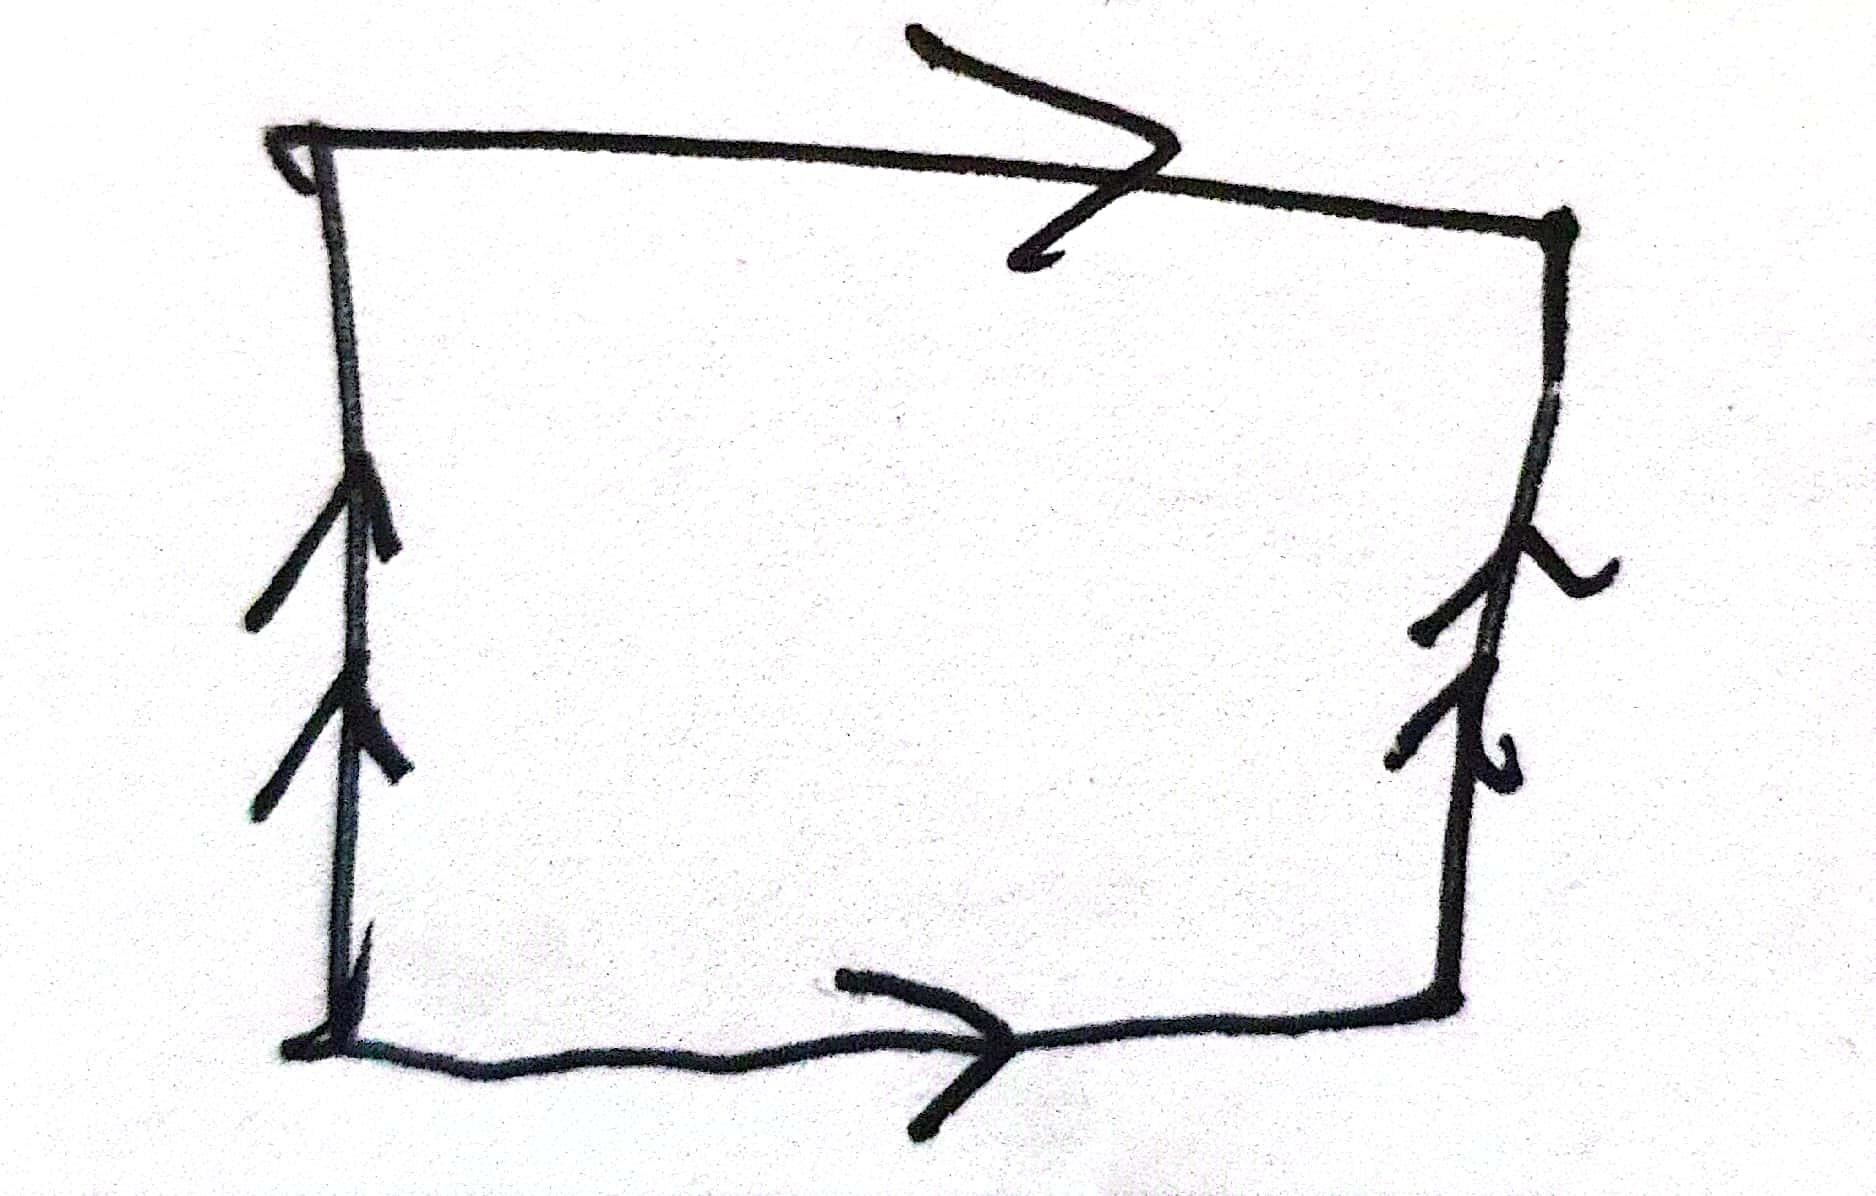
\includegraphics[width=0.3\textwidth]{7b.jpeg}
       \label{fig:7b-jpeg}
   \end{figure}
   Meridean circles correspond to vertical lines on the rectangle and
   longitudinal circles correspond to horizontal lines. By simply "cutting"
   along the meridian and longitudinal circles which we collapse, we can
   without loss of generality assume that the lines on the rectangle which we
   collapse are the borders of the rectangle.\\
   From here we have two reasonings which give the result:\\
   (1) The resulting space is a CW-complex with a $2$-cell attached to
   a $0$-cell which is $S^{2}$.\\
   \linebreak
   (2) Alternatively, we can note that the resulting space is a single point
   adjoined with $(0,1) \times (0,1)$. Now, as $I^2$ is compact as the product
   of compact spaces, so is the identification space. Furthermore, it is
   clearly Hausdorff and hence is the one-point compactification of $(0,1)
   \times (0,1)$. Now, as $(0,1) \times (0,1)$ is homeomorphic with
   $\mathbb{R}^2$ and one point compactifications are unique up to
   homeomorphism that differs only on the appended point, we have that
   the obtained identification space from the torus is the one-point
   compactification of $\mathbb{R}^2$ which is precisely
   $S^2$ (by stereographic projection).\\
   \linebreak
   (c) We claim that it is the wedge sum of two 2-spheres, $S^{2} \vee S^{2}$
   - i.e. a 2-sphere attached to another 2-sphere by a common point, or
   equivalently, the quotienting of two disjoint 2-spheres by identifying
   a point on each sphere.\\
   \linebreak
   To see this, suppose we divide the 2-sphere into two closed hemispheres
   - a northern and a southern one. The borders of the hemispheres are
   identified, and furthermore, the borders of the hemispheres are precisely
   the equator. So collapsing each border to a point, we find two separate
   CW-complexes of a $0$-cell with a $2$-cell attached, which is a sphere
   - this is simply $S^{2} = D^{2} / \partial D^{2}$. The
   $0$-cells are identified, giving the quotient of two disjoint 2-spheres by
   identifying a point on each sphere - i.e., we get  $S^{2} \vee S^{2}$.


   \begin{figure}[H]
       \centering
       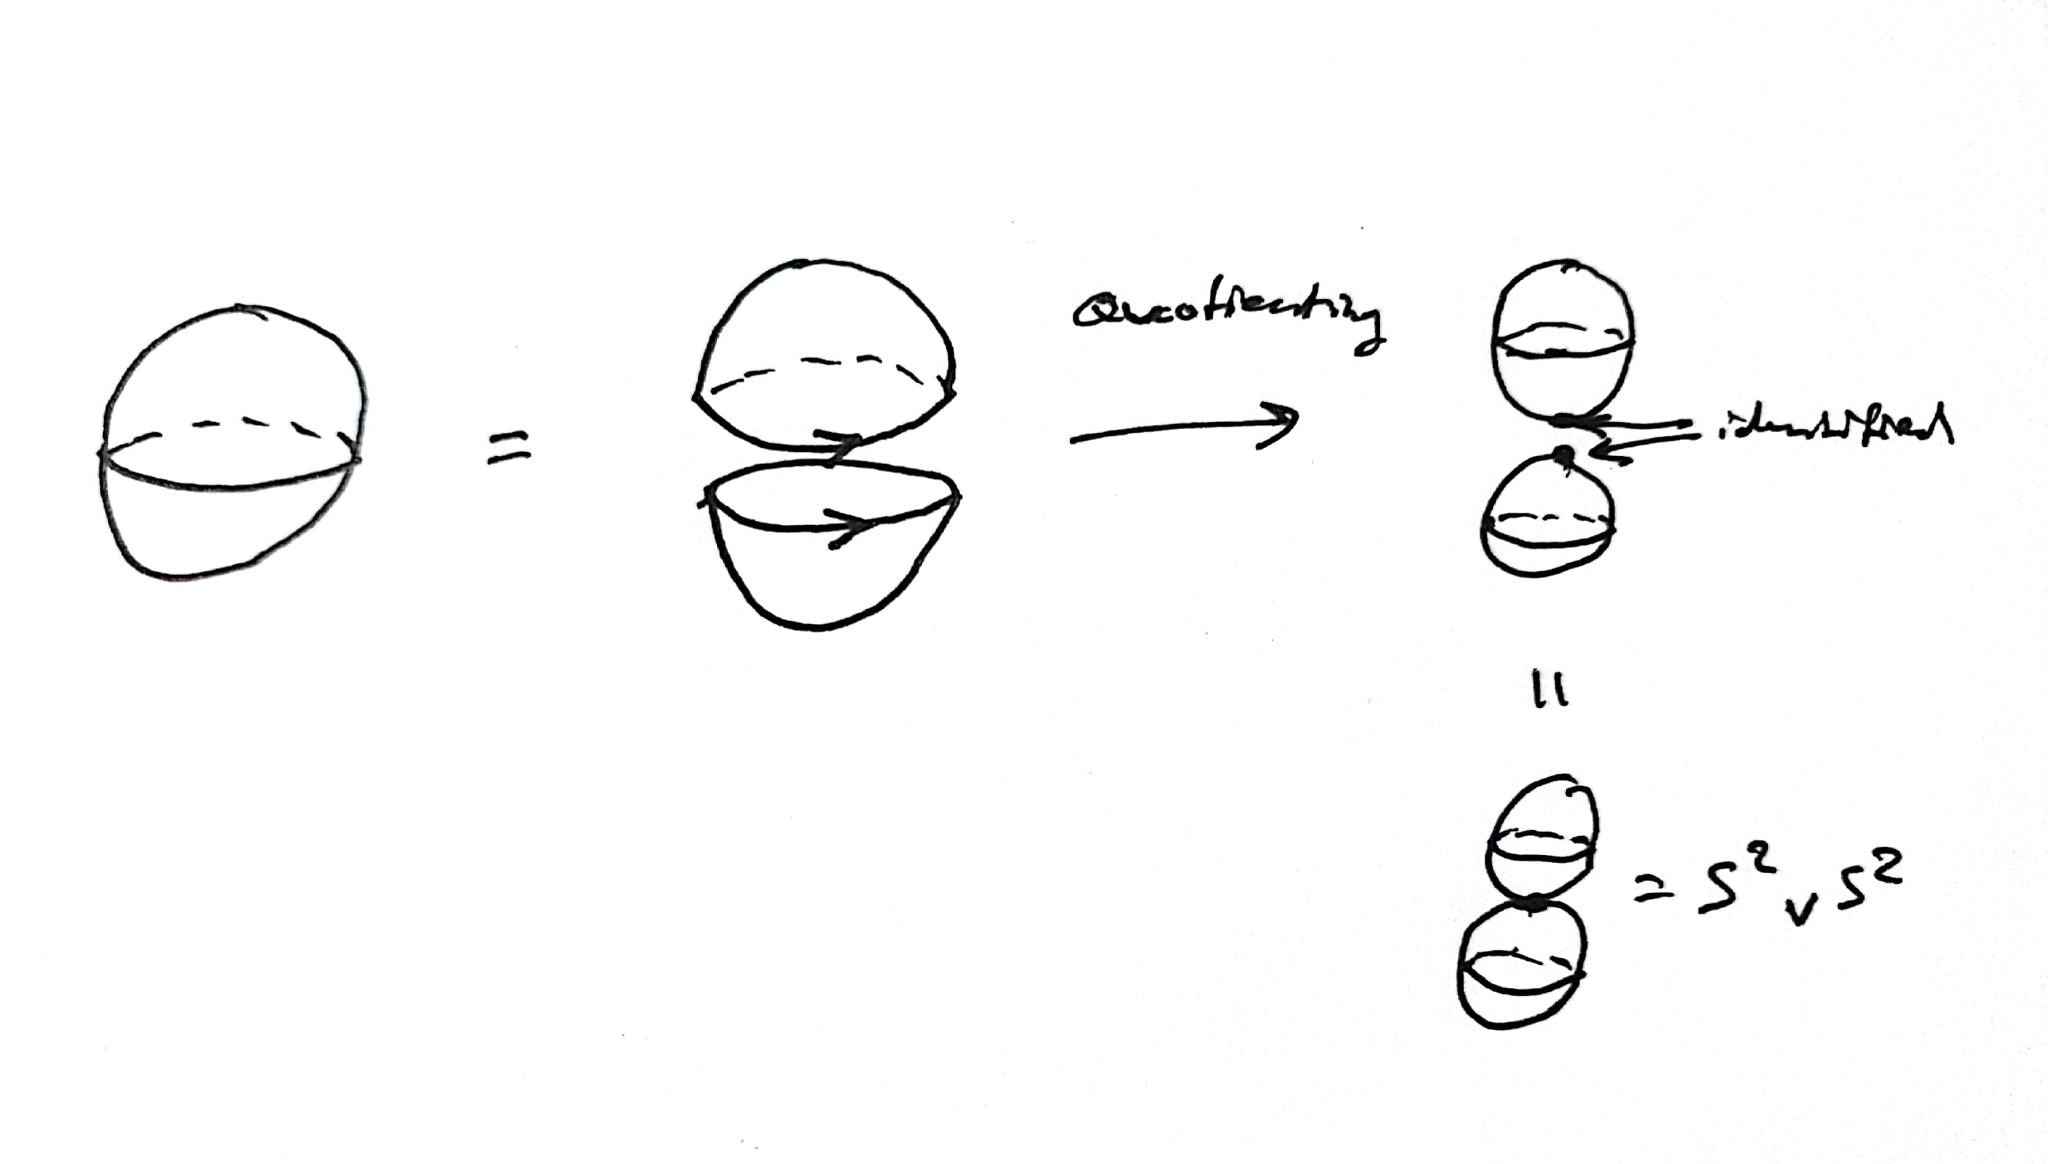
\includegraphics[width=0.8\textwidth]{3.jpeg}
       \label{fig:3-jpeg}
   \end{figure}

   (d) We claim that this is an infinite sequence of $2$-spheres, where
   each $2$-sphere is attached to two others at its north and south pole by a
   common point.\\
   To see this, let $X$ denote the identification space $\mathbb{R}^2$ with
   each
   circle centre the origin and of integer radius identified to its own
   point.\\
   Now, define maps
   $\varphi_n  \colon A_n \to S^{1} \times I$ where $A_n$ is the closed annulus 
   \[
   A_n = \left\{ x \in \mathbb{R}^2  \mid n \le \|x\| \le n+1 \right\},
   \] 
   by
   \[
   \varphi_n (x,y) = \left( \frac{(x,y)}{\|(x,y)\|}, \|(x,y)\|-n \right).
   \] 
   $\varphi_n$ is bijective, $A_n$ is compact and $S^{1} \times I$ is
   Hausdorff, hence $\varphi_n$ is a homeomorphism.\\
   Now, composing for each $n \ge 1$, $\varphi_n$ with the translation
   $S^{1} \times I \to S^{1} \left[ n, n+1 \right] $ by
   $(z,t) \to (z, t+ n)$, which is a homeomorphism. Now,
   $A_0$ is the closed disk with the boundary identified, which is the standard
   method of creating $S^{2}$. As we just showed,
   $\bigcup_{n \ge 1} A_n$ is homeomorphic to the infinite cylinder with base
   $S^{1}$: $S^{1} \times [ 1, \infty )$. Under this map, collapsing a circle
   with integer radius $n$ corresponds to collapsing the circle
   $S^{1} \times \left\{ n \right\} $, which, by considering the infinite
   cylinder as
   $S^{1} \times [1, \infty) = \bigcup_{n \in \mathbb{N}} S^{1} \times
   [n,n+1]$,
   gives by part (a) and theorem 4.2, that
   $X$ is homeomorphic with
   $S^{1} \times [0, \infty)$ with each $S^{1} \times \left\{ n \right\}
   $ identified to a point for each $n \in \mathbb{N}_0$.
   
   
\begin{figure}[H]
    \centering
    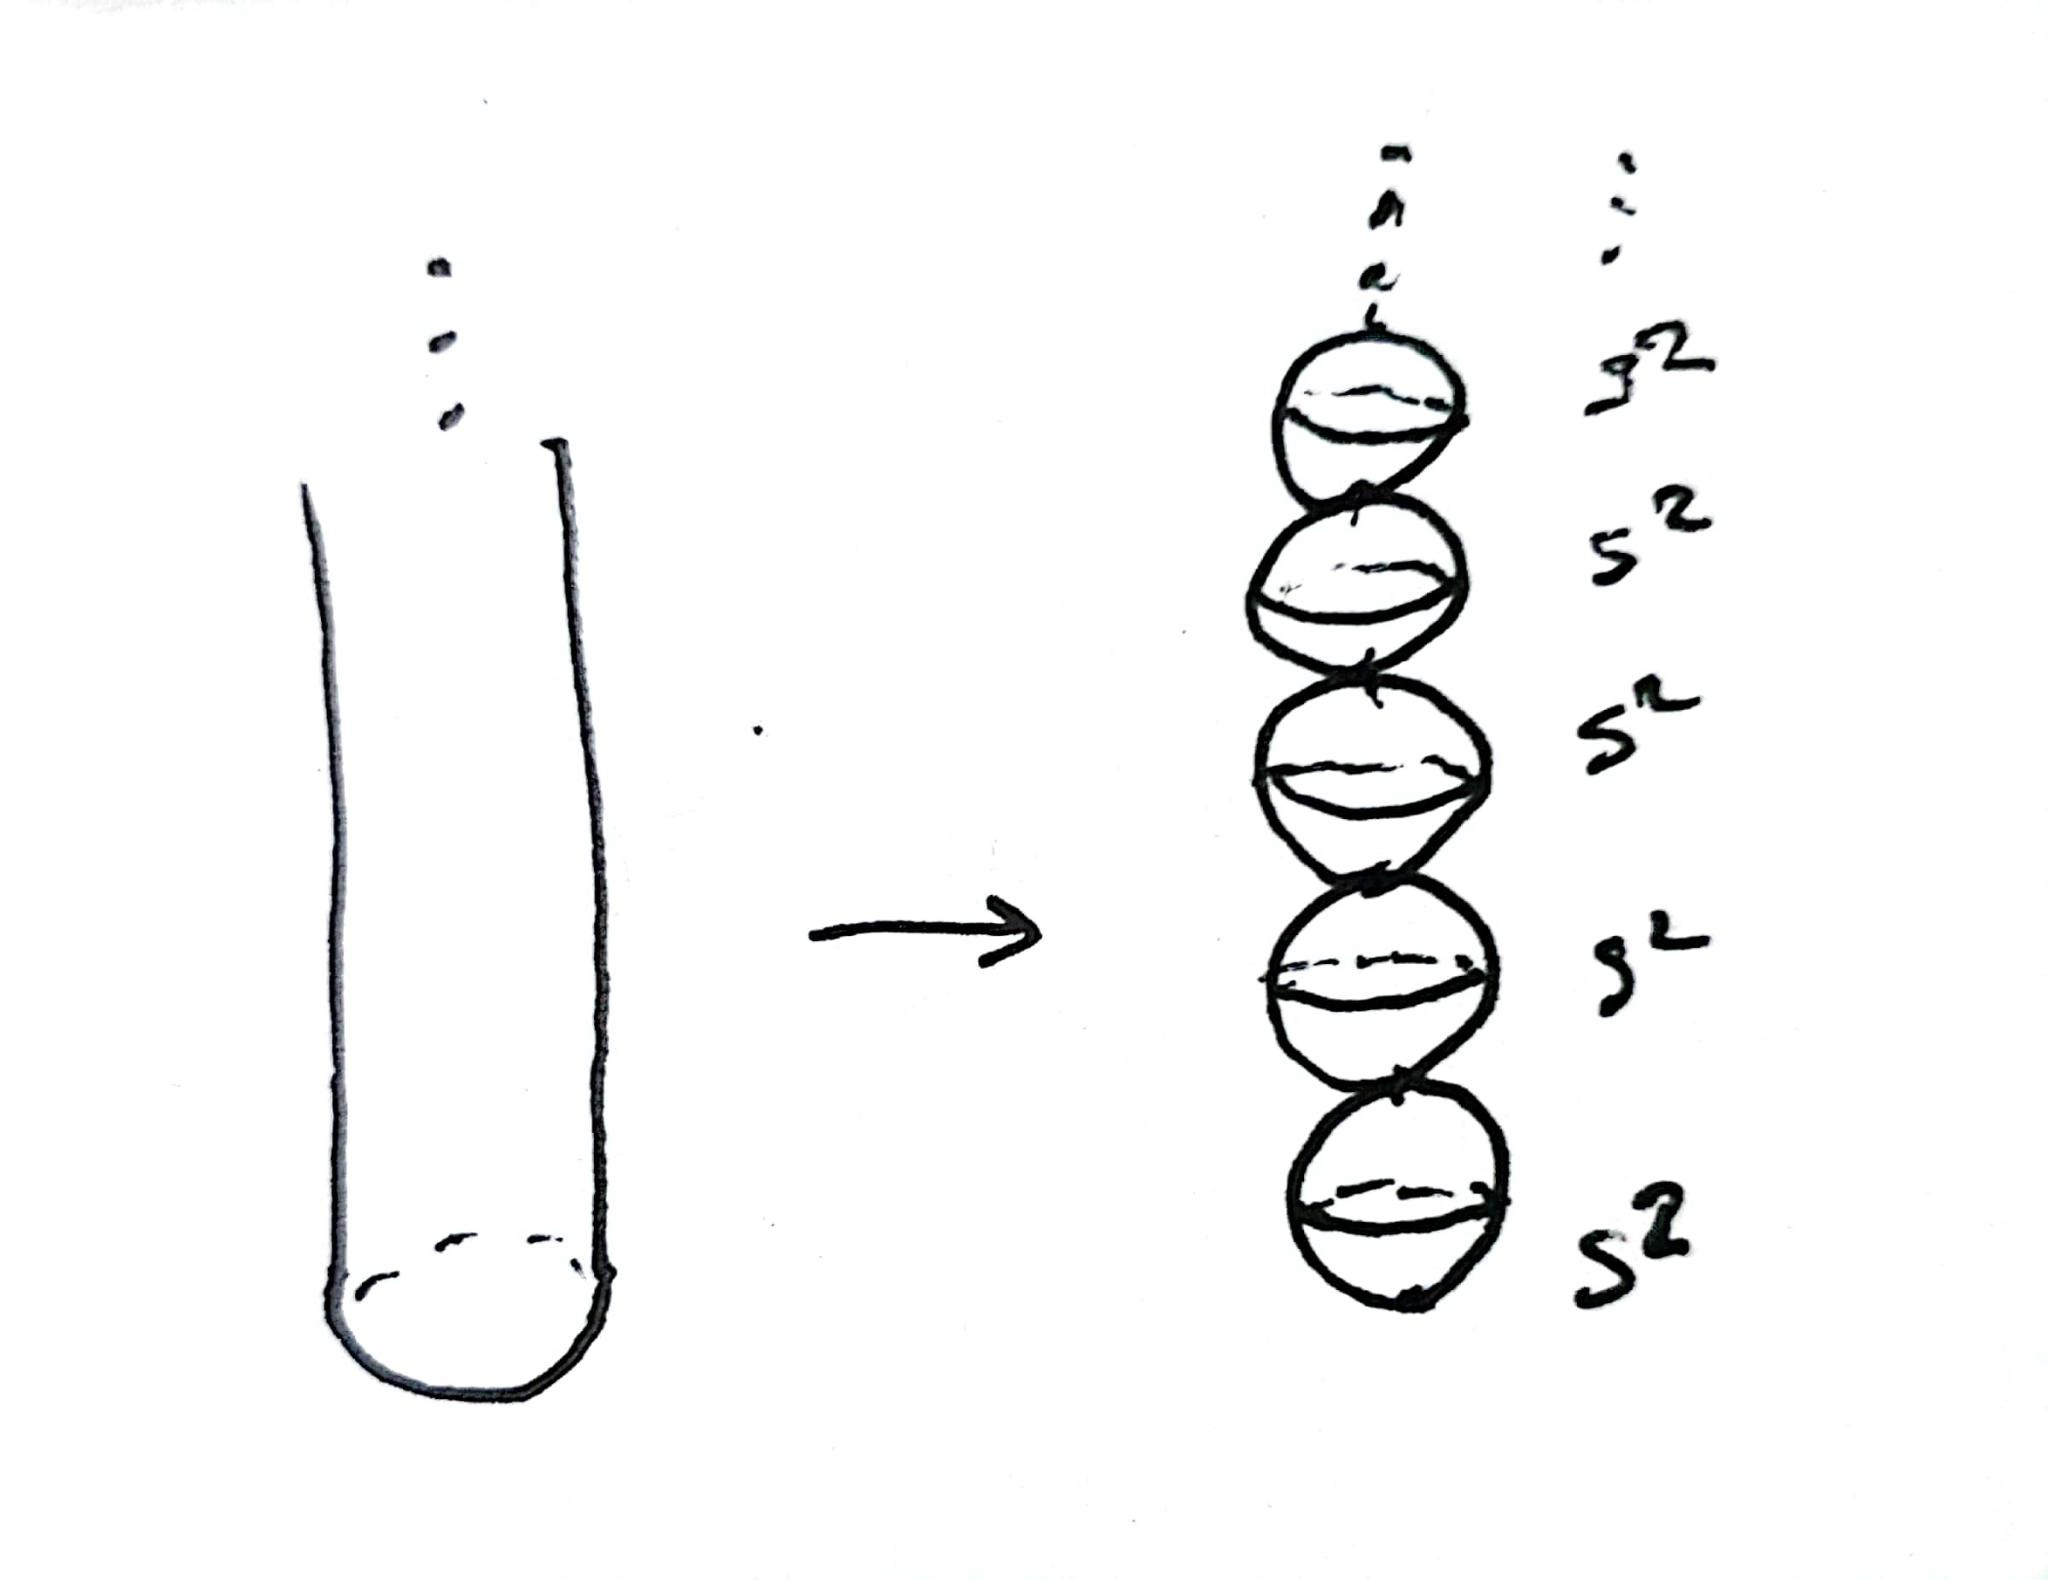
\includegraphics[width=0.5\textwidth]{4.jpeg}
    \label{fig:4-jpeg}
\end{figure}





























\end{document}
